\documentclass{article}

%%% Fill details here (in the second brackets)
\newcommand{\name}{Xin Qiu}     % Your name (First Last)
\newcommand{\wustlkey}{qiuxin}             % Your WUSTL Key
%%%



%%%%%%%%%%%%%%%%%%%%%% Formatting Stuff %%%%%%%%%%%%%%%%%%%%%%%%%%%
\usepackage{times}
\usepackage[T1]{fontenc}

\setlength{\parskip}{1em}\setlength{\parindent}{0pt}
\linespread{1.25}
\usepackage[margin=0.7in,top=1in]{geometry}\usepackage{fancyhdr}
\pagestyle{fancy}\lhead{\bf \name}\rhead{\bf \wustlkey}\cfoot{\thepage}
\newcommand{\info}{\clearpage \subsection*{Information}}
\newcommand{\solution}[1]{\clearpage \subsection*{Solution #1}}
\newcommand{\spart}[1]{\paragraph{(#1)}}
%%%%%%%%%%%%%%%%%%%%%%%%%%%%%%%%%%%%%%%%%%%%%%%%%%%%%%%%%%%%%%%%%%%


%%% Add any more packages if you want to
\usepackage{amsmath,graphicx}


\begin{document}
%%%%% Main Body goes here

% Begin solution to every problem like this.
\solution{1}
\spart{a} Based on the slides of lecture 6, the derivative of the cost function is:
$$
2(x - y) + \lambda|\cdot|
$$
then there are three ways to minimize the cost function as follows:
\begin{enumerate}
\item when $x > 0$, then we have $y - \frac{\lambda}{2} > 0$, so the minimum is $\lambda y + \frac{3\lambda^2}{4}$.
\item when $x < 0$, then we have $y + \frac{\lambda}{2} < 0$, so the minimum is $-\lambda y - \frac{\lambda^2}{4}$.
\item when $x = 0$, then we have $y - \frac{\lambda}{2} \le 0$ and $y + \frac{\lambda}{2} \ge 0$, so the minimum is $y^2$.
\end{enumerate}

\spart{b} Figure \ref{fig:prob1} shows the result of implementation of image denoising for problem 1.

\begin{figure*}[!h]
  \centering
    
\includegraphics[height=25em]{code/outputs/prob1.png}
  \caption{implementation of image denoising for problem 1.}
  \label{fig:prob1}
\end{figure*}

\solution{2} 
\spart{a} Figure \ref{fig:prob2a1} to Figure \ref{fig:prob2a3} show the result of the regular implementation of white-balanced with three factors computed to be inversely proportional to the mean three channels intensity in the image.

\begin{figure*}[!h]
  \centering
    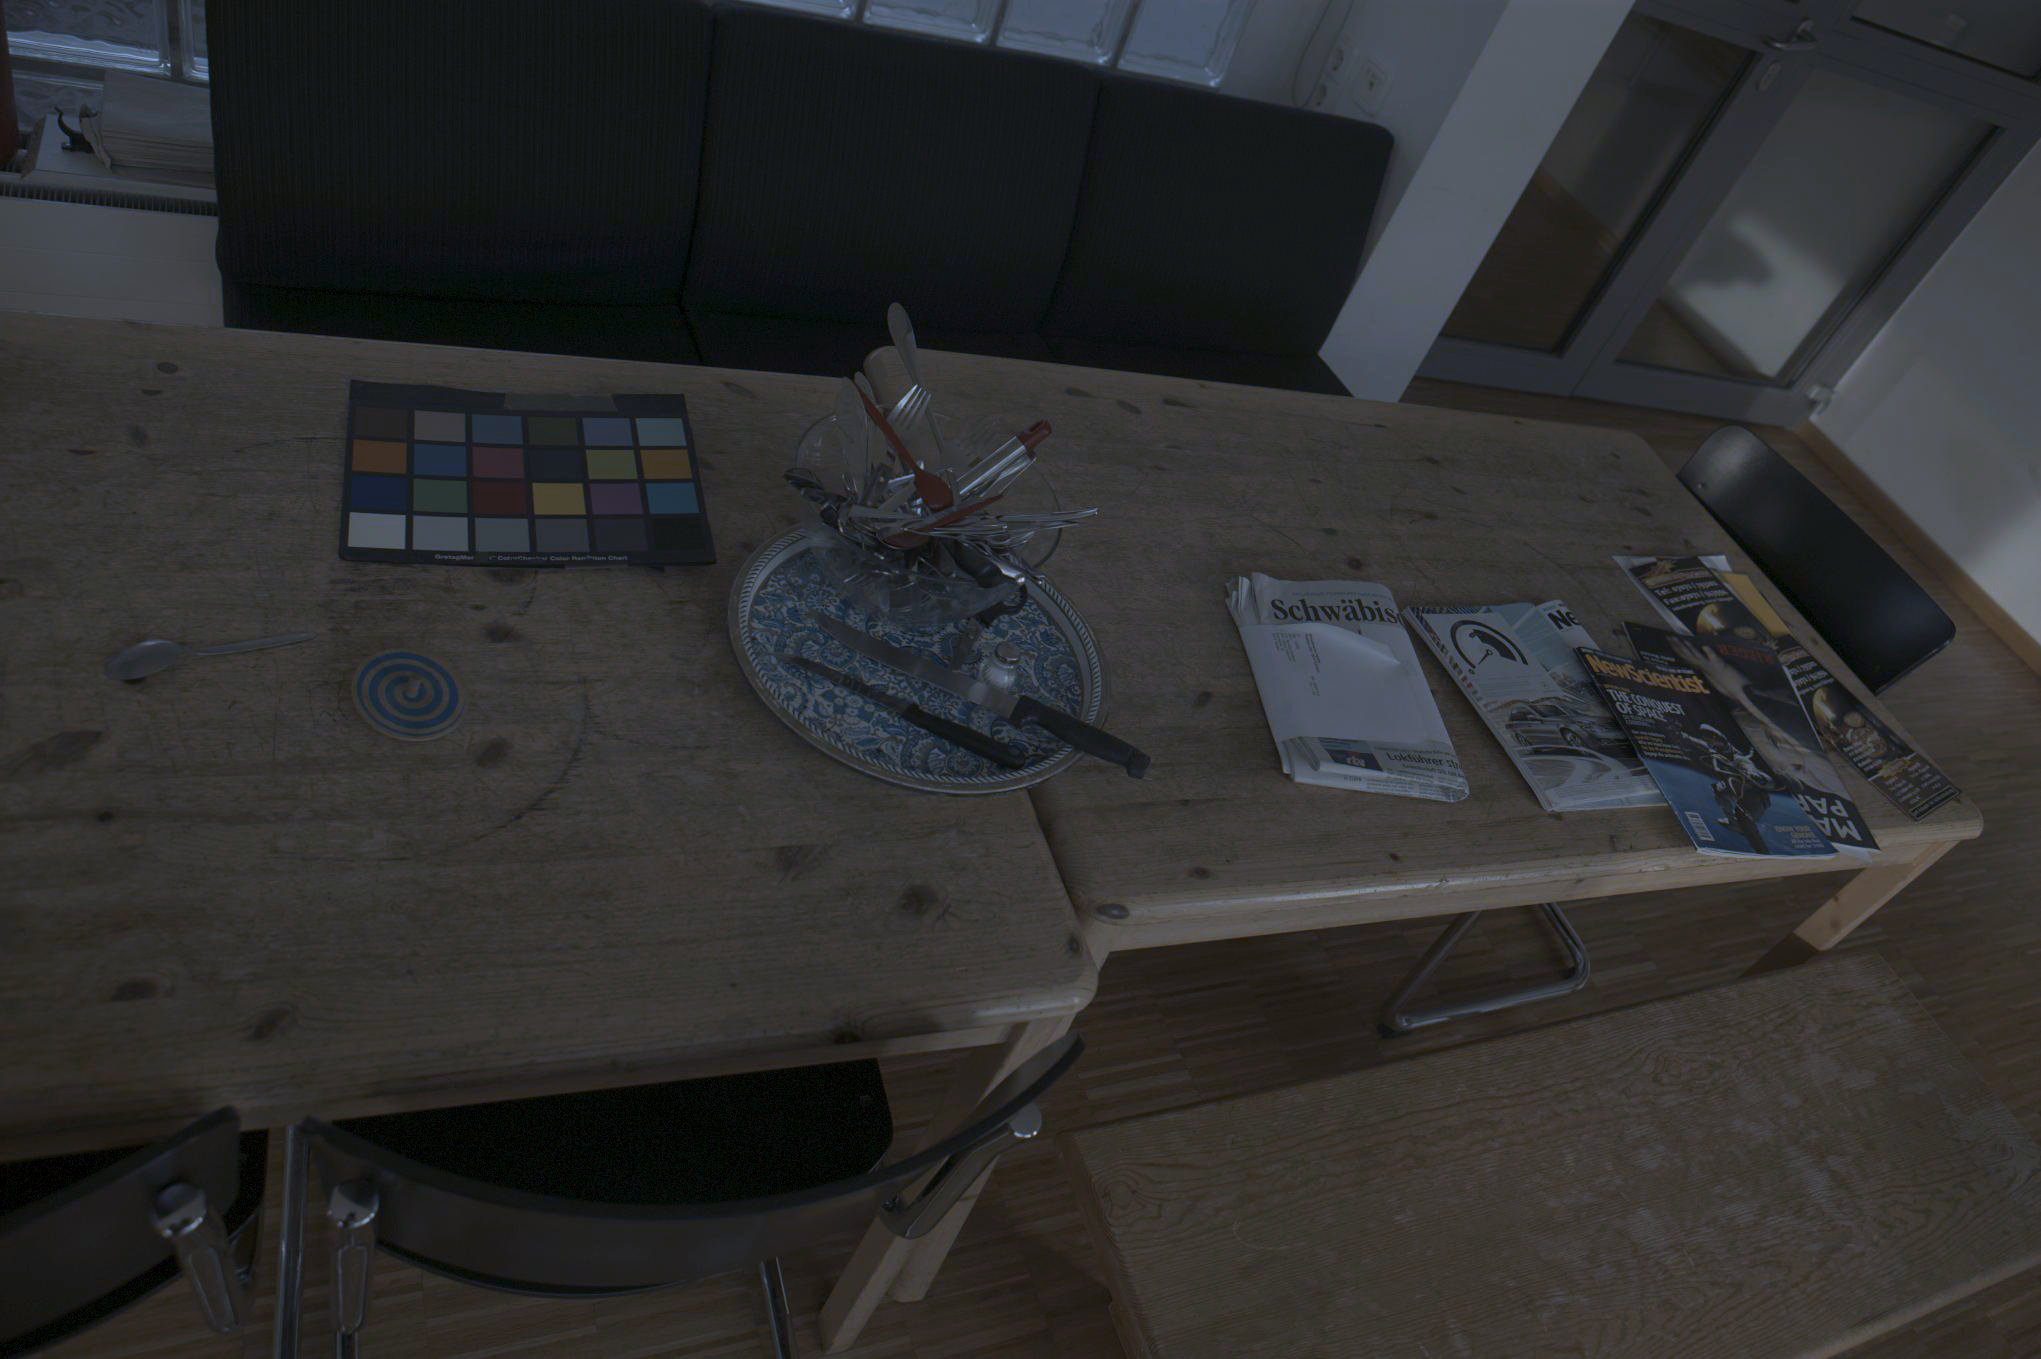
\includegraphics[height=25em]{code/outputs/prob2a_1.png}
  \caption{The regular implementation of white-balance}
  \label{fig:prob2a1}
\end{figure*}

\begin{figure*}[!h]
  \centering
    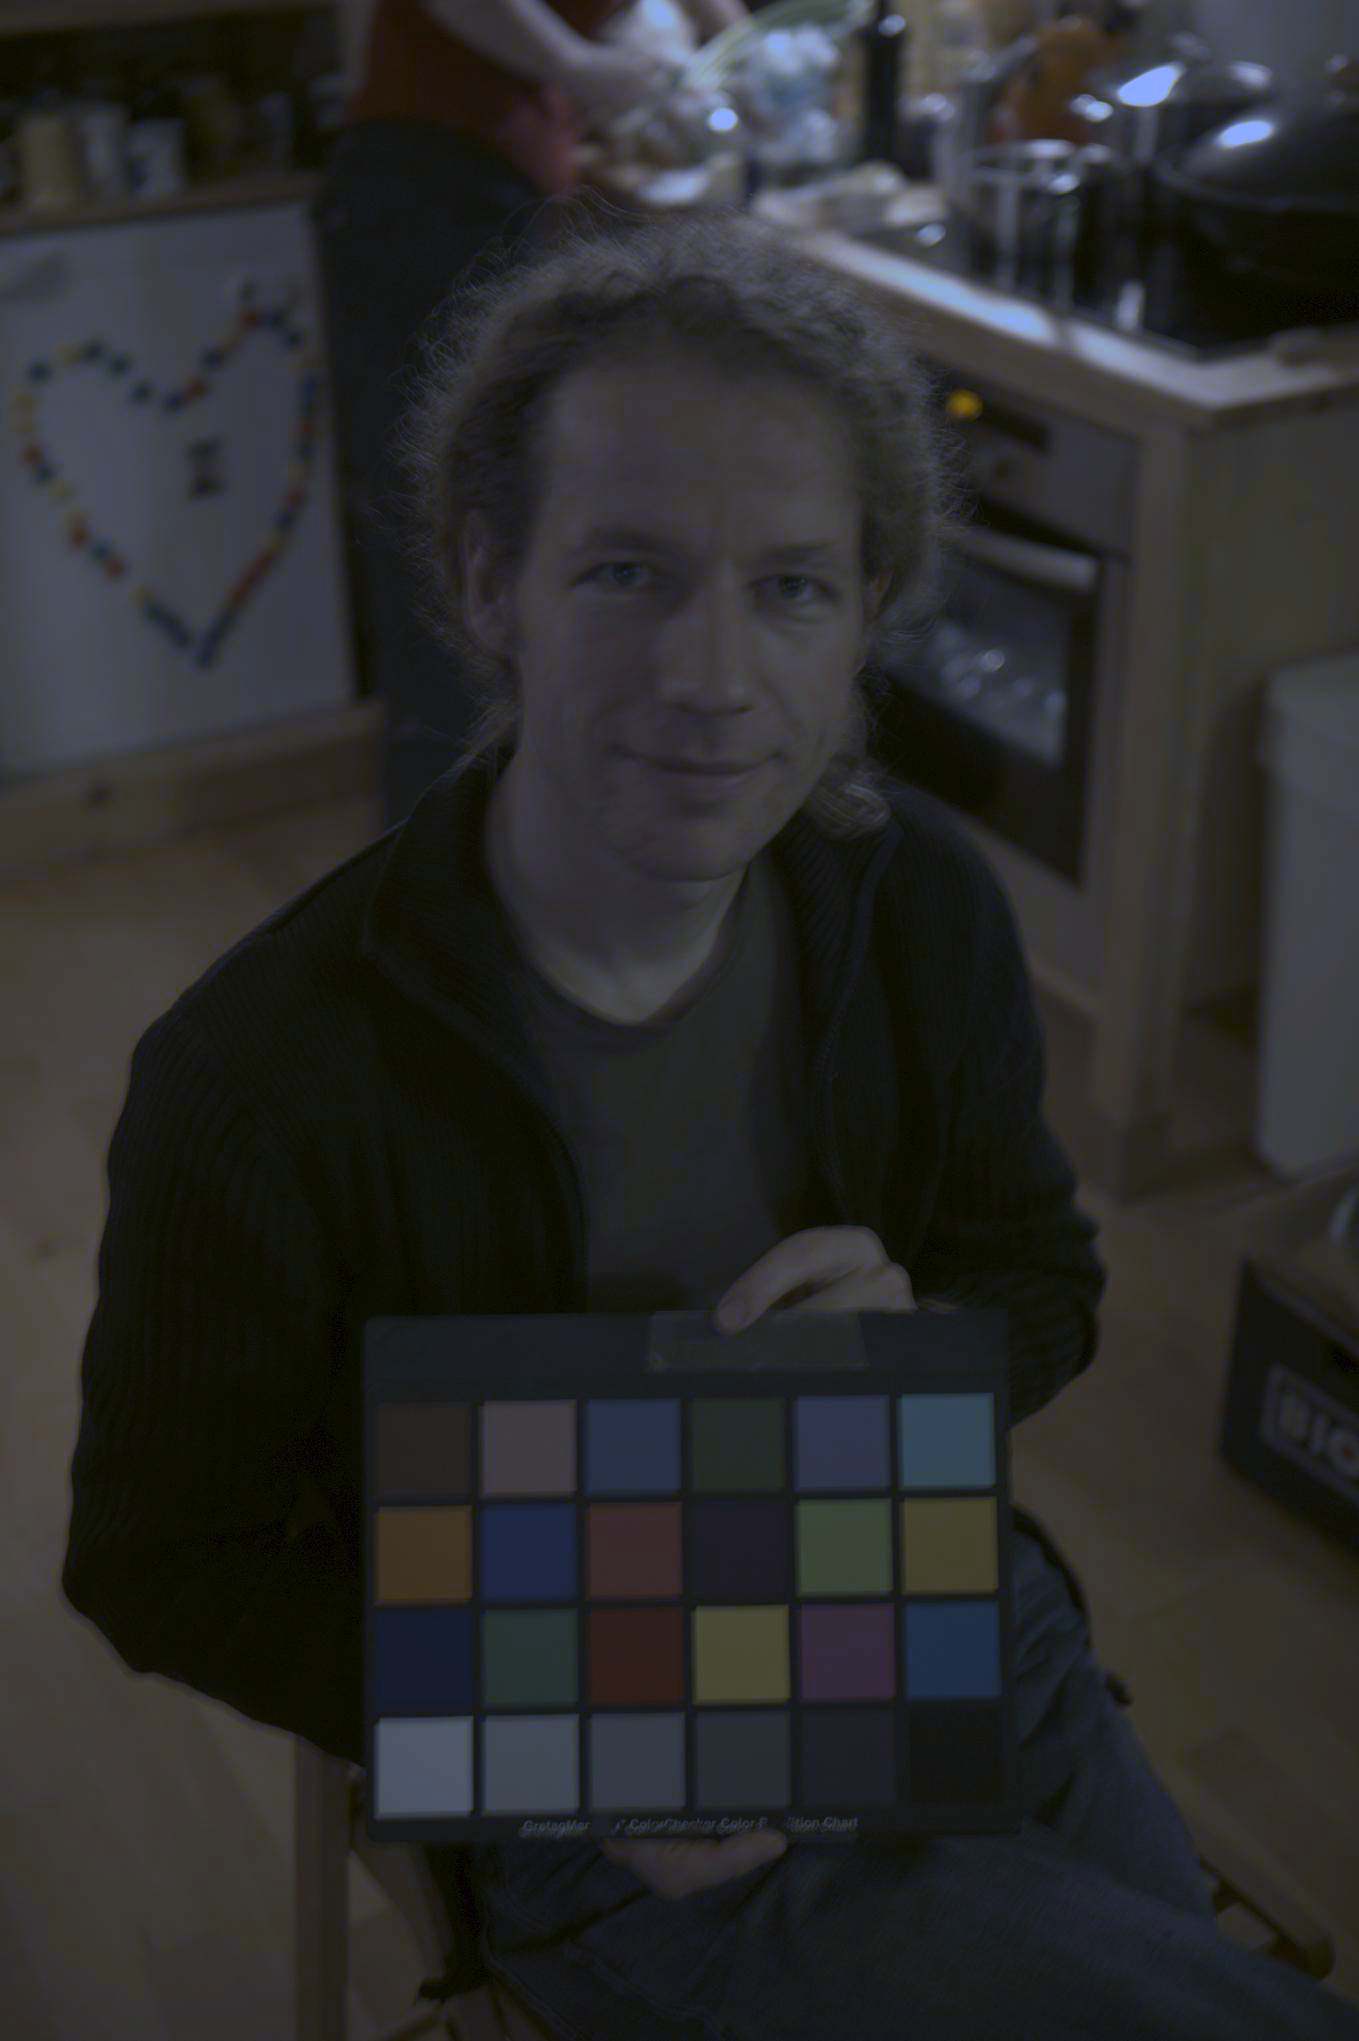
\includegraphics[height=25em]{code/outputs/prob2a_2.png}
  \caption{The regular implementation of white-balance}
  \label{fig:prob2a2}
\end{figure*}

\begin{figure*}[!h]
  \centering
    \includegraphics[height=25em]{code/outputs/prob2a_3.png}
  \caption{The regular implementation of white-balance}
  \label{fig:prob2a3}
\end{figure*}

\

\spart{b} Figure \ref{fig:prob2b1} to Figure \ref{fig:prob2b3} show the result of the implementation of white-balanced with three factors computed to be inversely proportional to averages over the 10\% brightest intensities in each channel.

\begin{figure*}[!h]
  \centering
    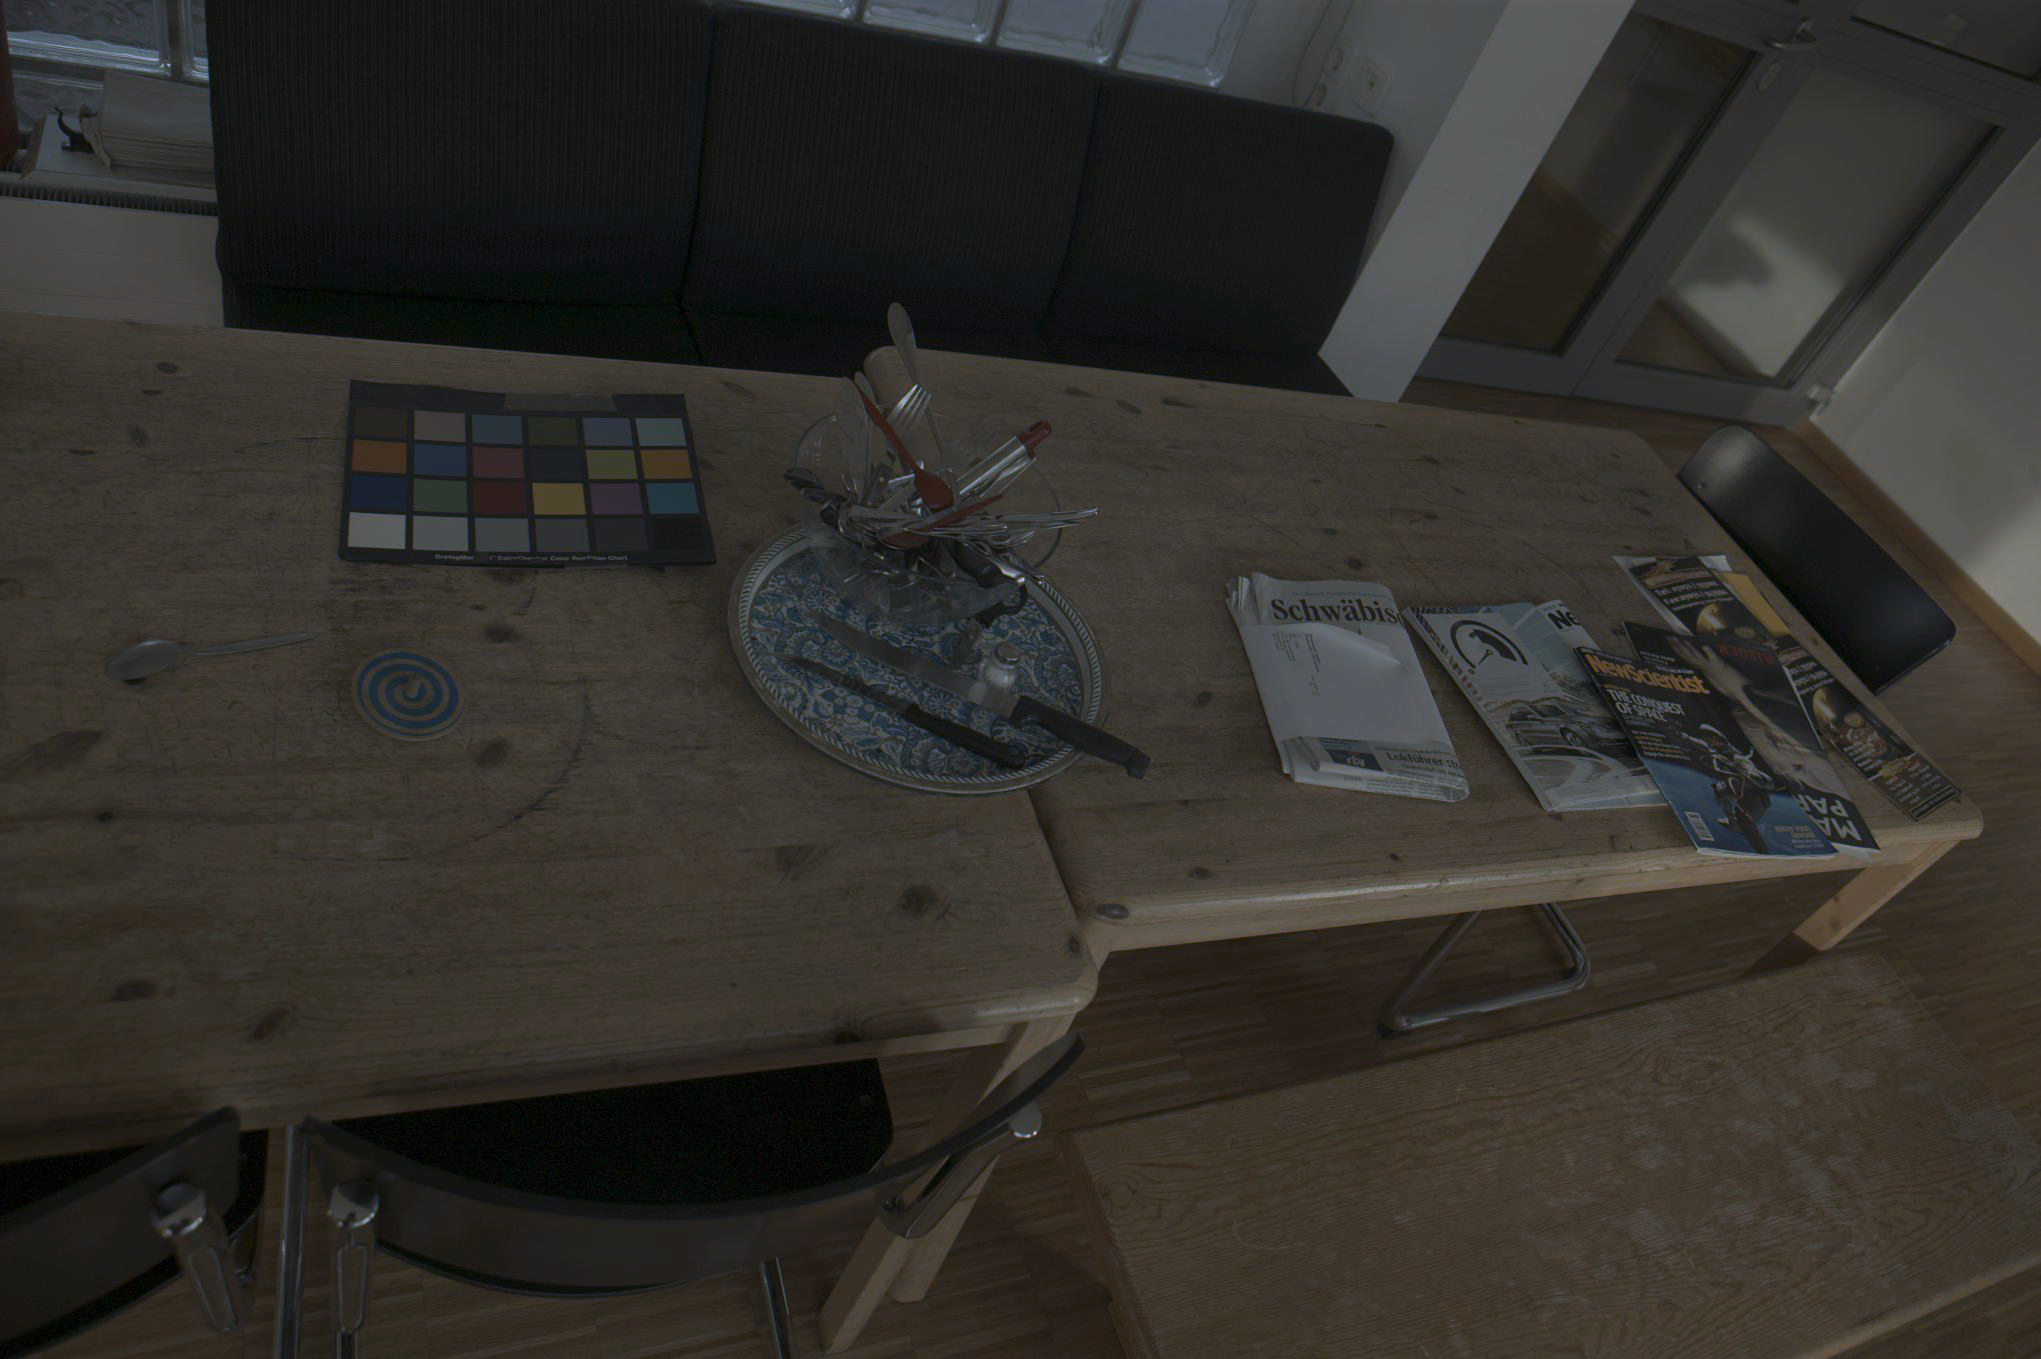
\includegraphics[height=25em]{code/outputs/prob2b_1.png}
  \caption{The implementation of white-balance with 10\% brightest intensities}
  \label{fig:prob2b1}
\end{figure*}

\begin{figure*}[!h]
  \centering
    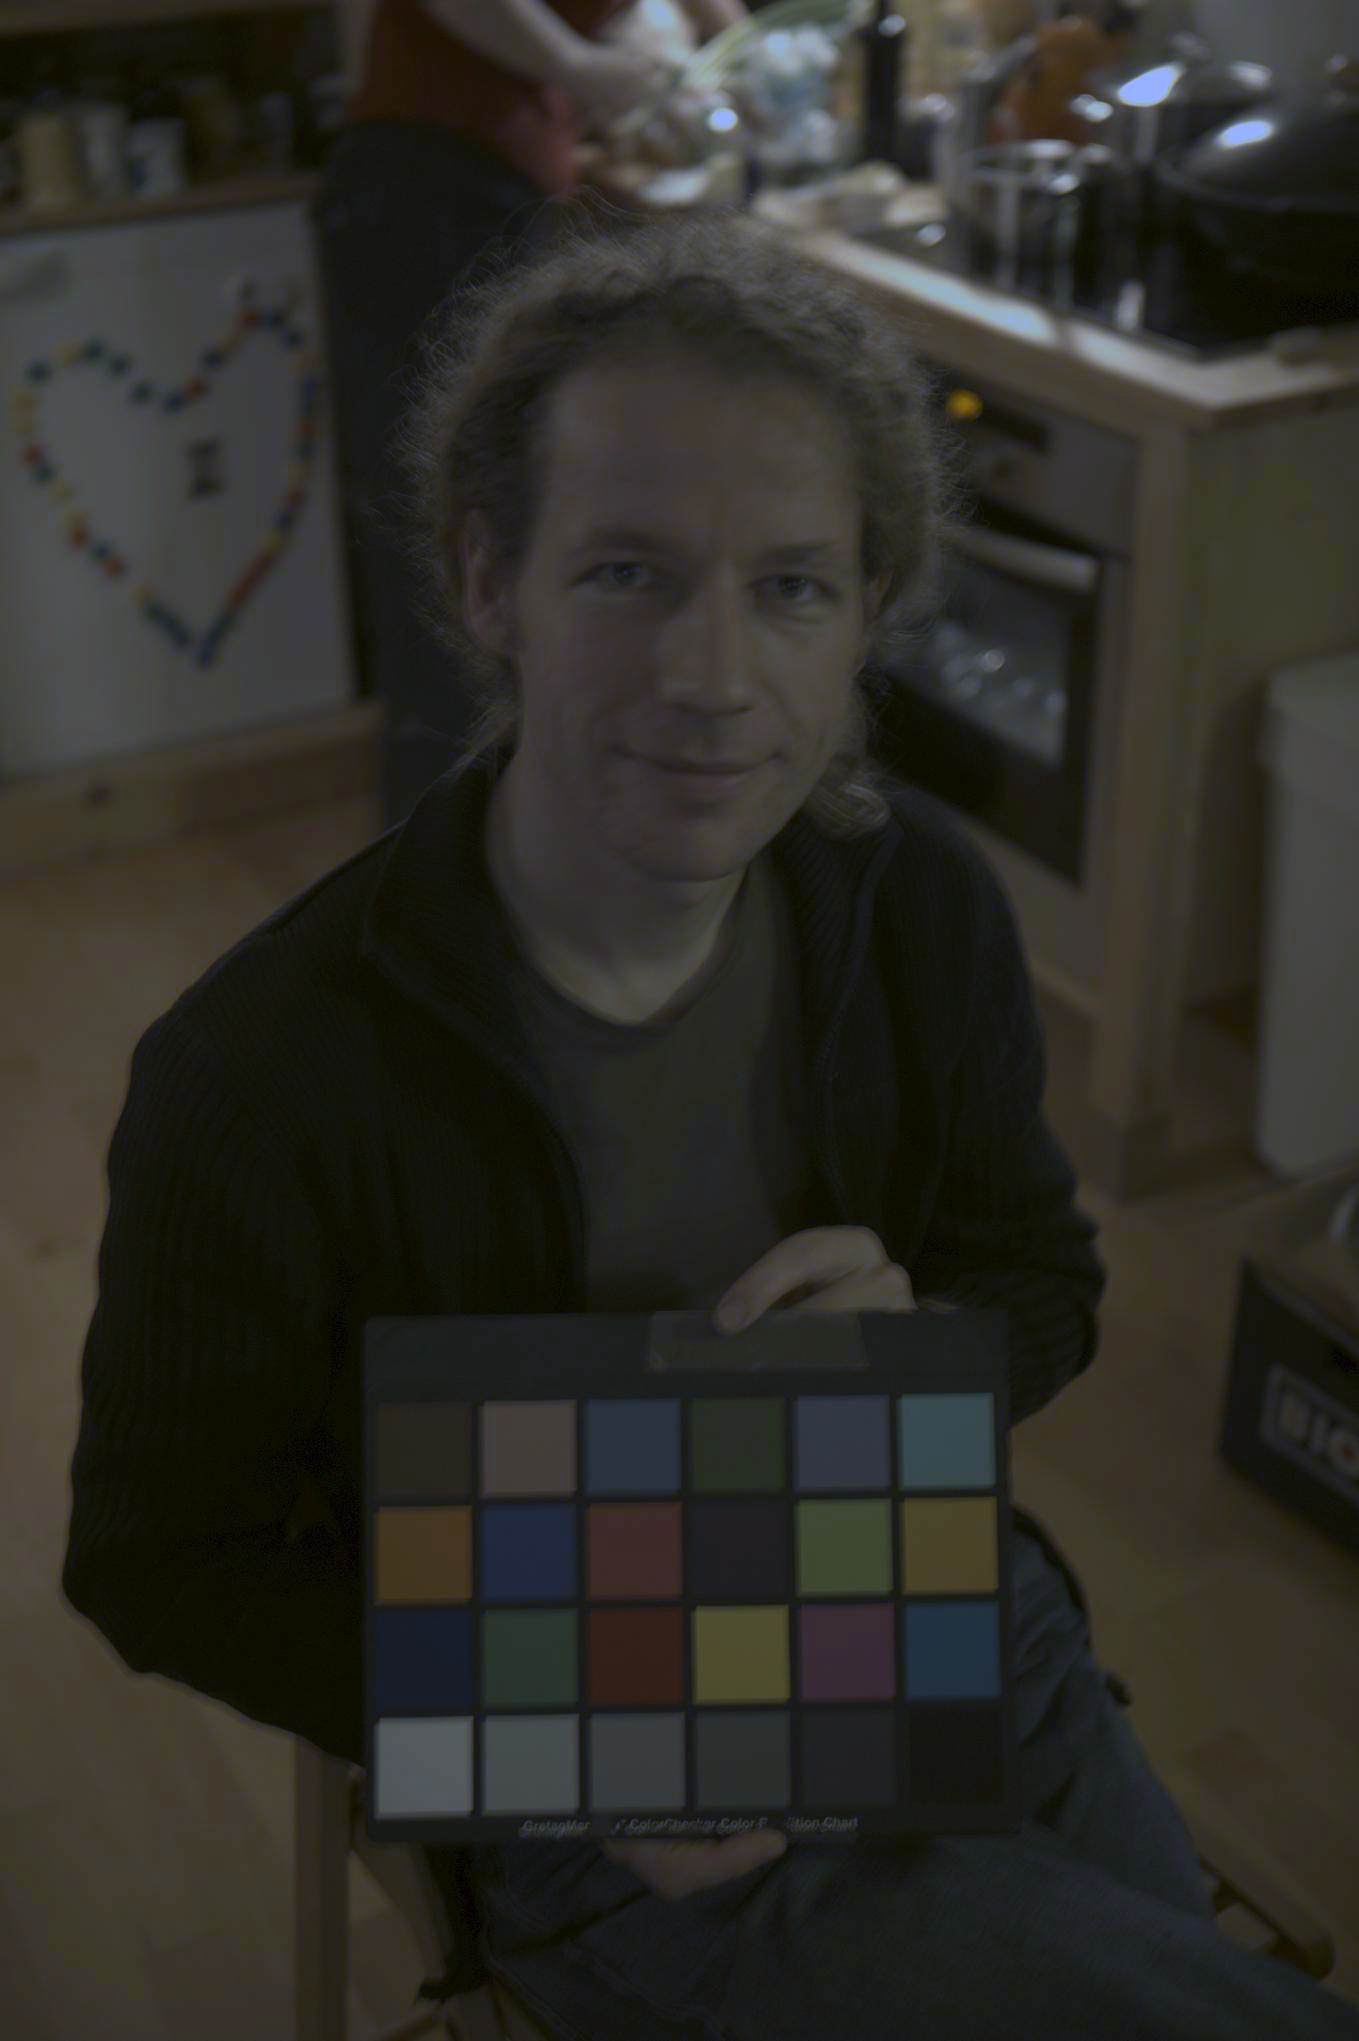
\includegraphics[height=25em]{code/outputs/prob2b_2.png}
  \caption{The implementation of white-balance with 10\% brightest intensities}
  \label{fig:prob2b2}
\end{figure*}

\begin{figure*}[!h]
  \centering
    \includegraphics[height=25em]{code/outputs/prob2b_3.png}
  \caption{The implementation of white-balance with 10\% brightest intensities}
  \label{fig:prob2b3}
\end{figure*}

\

\

 By observing the different between part (a) and part (b), I realized that the figures in part (a) are more affected by the dominant color then the figures in part (b). Take the first image as an example, the original image has so many green pixels, which presents too green. So, for the first algorithm, the mean value of green channel would be higher than red channel and blue channel, and more green intensity would be filter out when multiplied by the inverse mean. And also for the second algorithm, the three factors would be very close to 1 while we take the 10\% highest three colors intensity values, then as for the first image, less green intensity would be filter out. And images in part(b) are more closer to real images. This also works for the rest of two pairs.
 
 \solution{3}
 \spart{a} Figure \ref{fig:prob3a} shows the result of implementation photometric stereo as discussed in class for Lambertian surfaces.
 \begin{figure*}[!h]
  \centering
    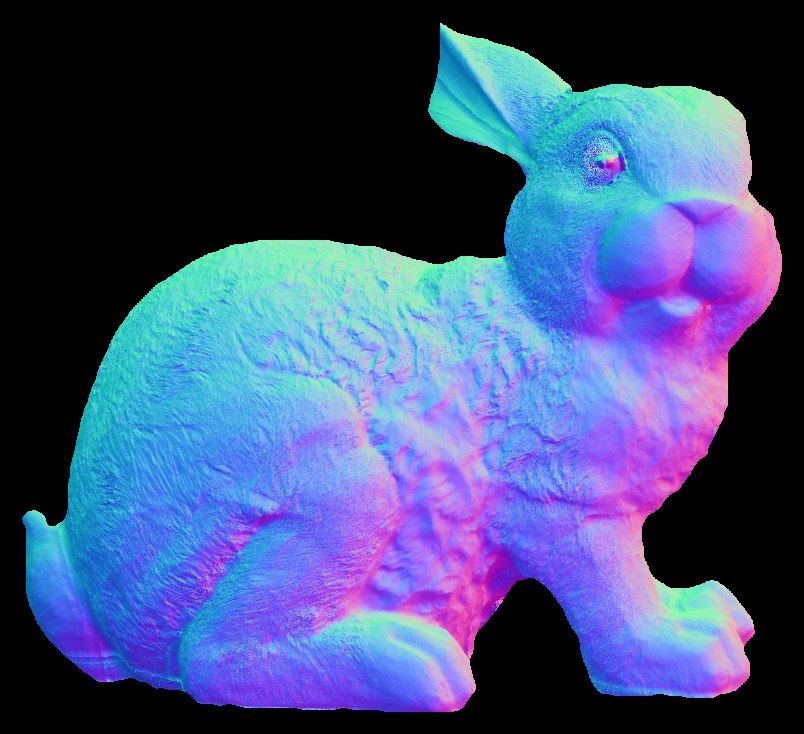
\includegraphics[height=23em]{code/outputs/prob3_nrm.png}
  \caption{The implementation of photometric stereo}
  \label{fig:prob3a}
\end{figure*}

\spart{b}Figure \ref{fig:prob3b} shows the result that computes an image of the surface color albedos.
\begin{figure*}[!h]
  \centering
    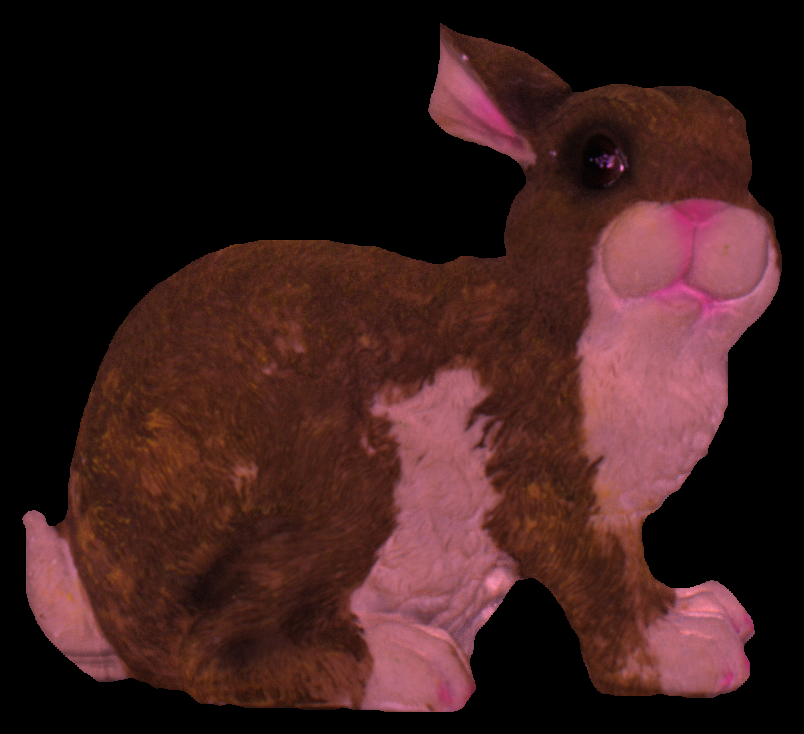
\includegraphics[height=23em]{code/outputs/prob3_alb.png}
  \caption{The implementation of computing an image of the surface color albedos}
  \label{fig:prob3b}
\end{figure*}

\solution{4} 
Implement the ntod function to compute a depth map. Figure \ref{fig:prob4} shows the result of it.
\begin{figure*}[!h]
  \centering
    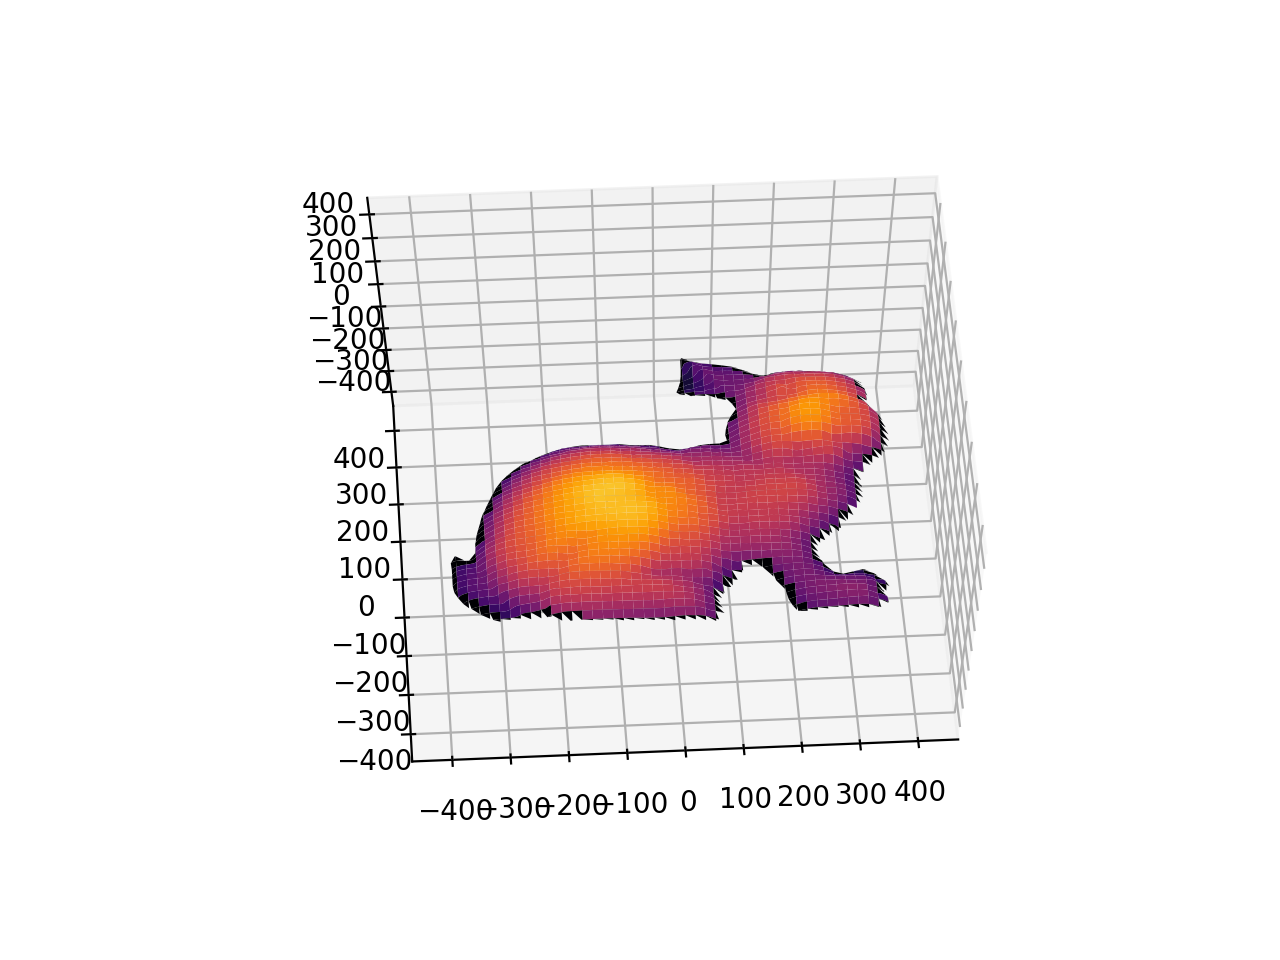
\includegraphics[height=30em]{code/outputs/prob4.png}
  \caption{The implementation of the ntod function to compute a depth map}
  \label{fig:prob4}
\end{figure*}

\solution{5}
Figure \ref{fig:prob5} shows the result of implementation of ntod function by using conjugate gradient.
\begin{figure*}[!h]
  \centering
    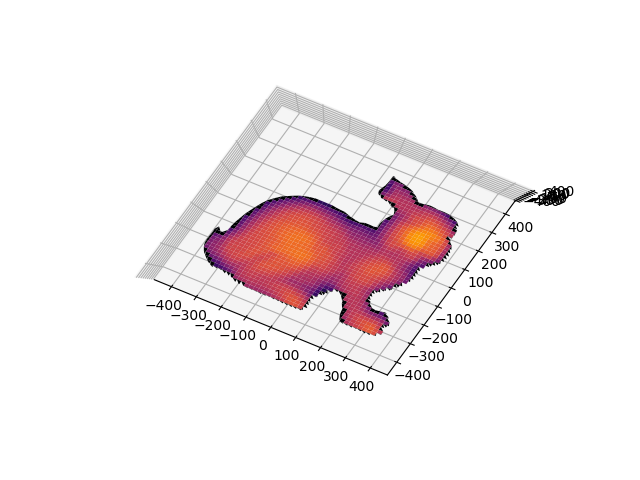
\includegraphics[height=30em]{code/outputs/prob5.png}
  \caption{The implementation of the ntod function by using conjugate gradient}
  \label{fig:prob5}
\end{figure*}




%%%%%%%%%% Important, you must edit and complete the informational
%%%%%%%%%% section below. If you discussed the problem set with no
%%%%%%%%%% one, edit it to say no discussions or external resources.
\info

This problem set took approximately 18 hours of effort.

I discussed this problem set with:
\begin{itemize}
\item Jiayao Cheng
\item Yukun Li
\end{itemize}

% Note that you might have to escape some special symbols in URLS like \_
I also got hints from the following sources:
\begin{itemize}
\item The slides from the class.
\item The recitation for the problem set and some hints from piazza.
\item Some hints and support code from pset1 solution key
\end{itemize}

\end{document}
